\documentclass[catalan,a4paper,twoside,11pt]{article}

\usepackage[T1]{fontenc}
\usepackage{mathpazo}
\usepackage[scaled=.95]{helvet}
\usepackage{courier}

\usepackage{amsmath, amssymb, amscd}
\usepackage{beccari-v2}

\usepackage{babel}
\usepackage{varioref}

\usepackage[final]{graphicx}

\usepackage{multicol}

\setlength{\parskip}{1.5ex plus0.5ex minus0.5ex}     % separaci\'{o} entre par\`{a}grafs
\setlength{\columnsep}{2em}                        % separaci\'{o} entre columnes
\setlength{\parindent}{0mm}

% format de les p\`{a}gines
\setlength{\hoffset}{0mm} \setlength{\oddsidemargin}{0mm}
\setlength{\evensidemargin}{-10.8mm} \setlength{\textwidth}{170mm}
\setlength{\marginparsep}{2mm} \setlength{\marginparwidth}{12mm}
\setlength{\voffset}{0mm} \setlength{\textheight}{230mm}
\setlength{\topmargin}{0mm}

\usepackage[pdftex=true,
bookmarks=true,bookmarksopenlevel=0,bookmarksopen=true,bookmarksnumbered=true,
pdftitle={\`{A}lgebra Vectorial},pdfauthor={Josep
Mollera},pdfview={FitH},pdfstartview={FitH}, pdfpagelabels=true,
colorlinks=true,linkcolor=blue,citecolor=blue,urlcolor=blue,plainpages=false]{hyperref}


\begin{document}

\title{\`{A}lgebra Vectorial v2.0}
\author{Josep Mollera Barriga}
\date{13 d'octubre de 2009}
\maketitle

\begin{multicols}{2}
\scriptsize \tableofcontents
\end{multicols}

\section{Definicions}

Es d\'{o}na  en primer lloc la definici\'{o} de les magnituds que
apareixen en les seccions seg\"{u}ents.

\begin{list}{}
{\setlength{\labelwidth}{14mm}
\setlength{\leftmargin}{16mm}\setlength{\labelsep}{2mm}}
   \item[$V$:] Volum d'integraci\'{o}.
   \item[$S$:]  Superf\'{\i}cie d'integraci\'{o}. $S$ \'{e}s la superf\'{\i}cie que
   limita el volum $V$.
   \item[$C$:] Corba d'integraci\'{o}. $C$ \'{e}s la corba tancada que
   limita la superf\'{\i}cie $S$.
   \item[$\diff\tau$:] Diferencial de volum, del volum V.
   \item[$\boldsymbol{\diff a}$:] Vector diferencial de superf\'{\i}cie, de la superf\'{\i}cie
   $S$. $\boldsymbol{\diff a}$ \'{e}s perpendicular a $S$.
   \item[$\boldsymbol{\diff l}$:] Vector diferencial de longitud, de la corba
   $C$. $\boldsymbol{\diff l}$ \'{e}s tangent a $C$.
   \item[$(x,y,z)$:] Coordenades d'un punt en un sistema de
   coordenades cartesianes.
   \item[$(\rho,\varphi,z)$:] Coordenades d'un punt en un sistema de
   coordenades cil\'{\i}ndriques.
   \item[$(r,\theta,\varphi)$:] Coordenades d'un punt en un sistema de
   coordenades esf\`{e}riques.
   \item[$\boldsymbol{\hat{\imath}},\boldsymbol{\hat{\jmath}},\boldsymbol{\hat{k}}$:]
   Vectors directors d'un sistema de  coordenades
   cartesianes.
   \item[$\boldsymbol{\hat{\rho}},\boldsymbol{\hat{\varphi}},\boldsymbol{\hat{z}}$:] Vectors directors d'un sistema de
   coordenades cil\'{\i}ndriques.
   \item[$\boldsymbol{\hat{r}},\boldsymbol{\hat{\theta}},\boldsymbol{\hat{\varphi}}$:] Vectors directors d'un sistema de
   coordenades esf\`{e}riques.
   \item[$P$:] Punt en $\mathbb{R}^3$.
   \item[$\boldsymbol{A,B,C}$:] Vectors en $\mathbb{R}^3$.
   \item[$\alpha$:] Angle entre dos vectors en $\mathbb{R}^3$.
   \item[$f,g$:] Funcions escalars; $f,g: \mathbb{R}^3\rightarrow\mathbb{R}$.
   \item[$\boldsymbol{F,G}$:] Funcions vectorials; $\boldsymbol{F,G}:\mathbb{R}^3\rightarrow\mathbb{R}^3$.
   \item[$\boldsymbol{\nabla}f$:] Gradient de la funci\'{o} escalar $f$;
   $\boldsymbol{\nabla}f:\mathbb{R}\rightarrow\mathbb{R}^3$
   \item[$\boldsymbol{\nabla\cdot F}$:] Diverg\`{e}ncia de la funci\'{o} vectorial $\boldsymbol{F}$;
   $\boldsymbol{\nabla\cdot F}: \mathbb{R}^3\rightarrow\mathbb{R}$.
   \item[$\boldsymbol{\nabla\times F}$:] Rotacional de la funci\'{o} vectorial $\boldsymbol{F}$;
   $\boldsymbol{\nabla\times F}:
   \mathbb{R}^3\rightarrow\mathbb{R}^3$.
   \item[$\boldsymbol{\nabla^2}f$:] Laplaci\`{a} de la funci\'{o} escalar $f$;
   $\boldsymbol{\nabla^2}f: \mathbb{R}\rightarrow\mathbb{R}$.
   \item[$\boldsymbol{\nabla^2F}$:] Laplaci\`{a} de la funci\'{o} vectorial $\boldsymbol{F}$; $\boldsymbol{\nabla^2F}: \mathbb{R}^3\rightarrow\mathbb{R}^3$.
\end{list}

\newcommand{\va}{\ensuremath{\,\boldsymbol{\hat{\imath}}}}
\newcommand{\vb}{\ensuremath{\,\boldsymbol{\hat{\jmath}}}}
\newcommand{\vc}{\ensuremath{\,\boldsymbol{\hat{k}}}}
\section{Sistemes de coordenades}

Es representen en la Figura \vref{pic:coord-cart-cil-esf}, tres dels
sistemes de coordenades m\'{e}s utilitzats: el cartesi\`{a}, el
cil\'{\i}ndric i l'esf\`{e}ric.

En el sistema de coordenades cartesianes, els vectors directors
tenen una orientaci\'{o} fixa, mentre que en els sistemes de
coordenades cil\'{\i}ndriques i esf\`{e}riques, els vectors
directors tenen una orientaci\'{o} variable, que dep\`{e}n del punt
$P$ al qual ens estiguem referint.
\begin{figure}[h]
\centering
   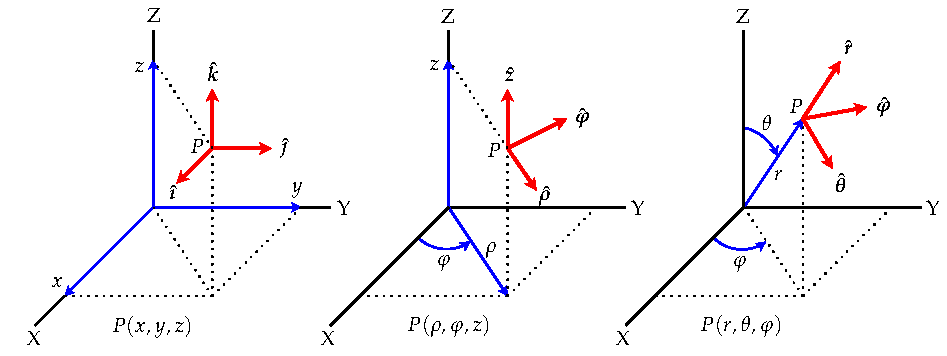
\includegraphics{Imatges/Coordenades.pdf}
\caption{Coordenades cartesianes, cil\'{\i}ndriques i esf\`{e}riques}
\label{pic:coord-cart-cil-esf}
\end{figure}

Els rangs de les coordenades de cadascun del tres sistemes s\'{o}n:
\begin{align}
    &\text{Cartesianes:} & & x\in(-\infty,\infty) & &
    y\in(-\infty,\infty) & & z\in(-\infty,\infty) \\
    &\text{Cil\'{\i}ndriques:} & & \rho\in[0,\infty) & &
    \varphi\in[0,2\pi) & & z\in(-\infty,\infty) \\
    &\text{Esf\`{e}riques:} & & r\in[0,\infty) & &
    \theta\in[0,\pi] & & \varphi\in[0,2\pi)
\end{align}

\subsection{Relacions entre les coordenades cartesianes i
cil\'{\i}ndriques}

Les coordenades cartesianes  d'un punt $P(x,y,z)$, s'obtenen partir
de les seves coordenades cil\'{\i}ndriques $P(\rho,\varphi,z)$,
mitjan\c{c}ant les relacions seg\"{u}ents:
\begin{subequations}\begin{align}
    x &=\rho\cos\varphi \\ y &=\rho\sin\varphi \\ z &=z
\end{align}\end{subequations}

Les coordenades  cil\'{\i}ndriques  d'un punt $P(\rho,\varphi,z)$,
s'obtenen partir de les seves coordenades cartesianes $P(x,y,z)$,
mitjan\c{c}ant les relacions seg\"{u}ents:
\begin{subequations}\begin{align}
    \rho &= \sqrt{x^2+y^2}\\
    \varphi &=  \arctan\frac{y}{x}\\
    z &= z
\end{align}\end{subequations}

L'expressi\'{o} en coordenades cartesianes dels vectors directors d'un sistema de coordenades  cil\'{\i}ndriques $\boldsymbol{\hat{\rho}},\boldsymbol{\hat{\varphi}},\boldsymbol{\hat{z}}$ \'{e}s:
\begin{subequations}\begin{align}
    \boldsymbol{\hat{\rho}} &=\cos\varphi\va+\sin\varphi\vb \\
    \boldsymbol{\hat{\varphi}} &=-\sin\varphi\va+\cos\varphi\vb \\
    \boldsymbol{\hat{z}} &=\vc
\end{align}\end{subequations}

L'expressi\'{o} en coordenades cil\'{\i}ndriques dels vectors directors d'un sistema de coordenades  cartesianes $\va,\vb,\vc$ \'{e}s:
\begin{subequations}\begin{align}
    \va &=\cos\varphi\,\boldsymbol{\hat{\rho}}-\sin\varphi\,\boldsymbol{\hat{\varphi}} \\
    \vb &=\sin\varphi\,\boldsymbol{\hat{\rho}}+\cos\varphi\,\boldsymbol{\hat{\varphi}} \\
    \vc &=\boldsymbol{\hat{z}}
\end{align}\end{subequations}

\subsection{Relacions entre les coordenades cartesianes i
esf\`{e}riques}

Les coordenades cartesianes  d'un punt $P(x,y,z)$, s'obtenen partir
de les seves coordenades esf\`{e}riques $P(r,\theta,\varphi)$,
mitjan\c{c}ant les relacions seg\"{u}ents:
\begin{subequations}\begin{align}
    x &=r\sin\theta\cos\varphi \\ y &=r\sin\theta\sin\varphi \\ z &=r\cos\theta
\end{align}\end{subequations}

Les coordenades  esf\`{e}riques  d'un punt $P(r,\theta,\varphi)$,
s'obtenen partir de les seves coordenades cartesianes $P(x,y,z)$,
mitjan\c{c}ant les relacions seg\"{u}ents:
\begin{subequations}\begin{align}
    r &=\sqrt{x^2+y^2+z^2}\\
    \theta&=\arccos\frac{z}{\sqrt{x^2+y^2+z^2}}\\
    \varphi &=\arctan\frac{y}{x}
\end{align}\end{subequations}


L'expressi\'{o} en coordenades cartesianes dels vectors directors d'un sistema de coordenades  esf\`{e}riques $\boldsymbol{\hat{r}},\boldsymbol{\hat{\theta}},\boldsymbol{\hat{\varphi}}$ \'{e}s:
\begin{subequations}\begin{align}
    \boldsymbol{\hat{r}} &=\sin\theta\cos\varphi\va+ \sin\theta\sin\varphi\vb+\cos\theta\vc\\
    \boldsymbol{\hat{\theta}} &=\cos\theta\cos\varphi\va+
    \cos\theta\sin\varphi\vb-\sin\theta\vc\\
    \boldsymbol{\hat{\varphi}}&=-\sin\varphi\va+\cos\varphi\vb
\end{align}\end{subequations}

L'expressi\'{o} en coordenades esf\`{e}riques dels vectors directors d'un sistema de coordenades  cartesianes $\va,\vb,\vc$ \'{e}s:
\begin{subequations}\begin{align}
    \va &=\sin\theta\cos\varphi\,\boldsymbol{\hat{r}}+
    \cos\theta\cos\varphi\,\boldsymbol{\hat{\theta}}-\sin\varphi\,\boldsymbol{\hat{\varphi}}\\
    \vb &=\sin\theta\sin\varphi\,\boldsymbol{\hat{r}}+
    \cos\theta\sin\varphi\,\boldsymbol{\hat{\theta}}+\cos\varphi\,\boldsymbol{\hat{\varphi}}\\
    \vc &=\cos\theta\,\boldsymbol{\hat{r}}-\sin\theta\,\boldsymbol{\hat{\theta}}
\end{align}\end{subequations}

\subsection{Relacions entre les coordenades cil\'{\i}ndriques i
esf\`{e}riques}

Les coordenades cil\'{\i}ndriques  d'un punt $P(\rho,\varphi,z)$,
s'obtenen partir de les seves coordenades esf\`{e}riques
$P(r,\theta,\varphi)$, mitjan\c{c}ant les relacions seg\"{u}ents:
\begin{subequations}\begin{align}
    \rho &=r\sin\theta \\ \varphi &=\varphi \\z &=r\cos\theta
\end{align}\end{subequations}

Les coordenades  esf\`{e}riques  d'un punt $P(r,\theta,\varphi)$,
s'obtenen partir de les seves coordenades cil\'{\i}ndriques
$P(\rho,\varphi,z)$, mitjan\c{c}ant les relacions seg\"{u}ents:
\begin{subequations}\begin{align}
    r &=\sqrt{\rho^2+z^2}\\
    \theta &=\arctan\frac{\rho}{z}\\
    \varphi &=\varphi
\end{align}\end{subequations}

L'expressi\'{o} en coordenades cil\'{\i}ndriques dels vectors directors d'un sistema de coordenades  esf\`{e}riques $\boldsymbol{\hat{r}},\boldsymbol{\hat{\theta}},\boldsymbol{\hat{\varphi}}$ \'{e}s:
\begin{subequations}\begin{align}
    \boldsymbol{\hat{r}} &=\sin\theta\,\boldsymbol{\hat{\rho}}+\cos\theta\,\boldsymbol{\hat{z}}\\
    \boldsymbol{\hat{\theta}}
    &=\cos\theta\,\boldsymbol{\hat{\rho}}-\sin\theta\,\boldsymbol{\hat{z}}\\
    \boldsymbol{\hat{\varphi}}&=\boldsymbol{\hat{\varphi}}
\end{align}\end{subequations}

L'expressi\'{o} en coordenades esf\`{e}riques dels vectors directors d'un sistema de coordenades  cil\'{\i}ndriques $\boldsymbol{\hat{\rho}},\boldsymbol{\hat{\varphi}},\boldsymbol{\hat{\theta}}$ \'{e}s:
\begin{subequations}\begin{align}
    \boldsymbol{\hat{\rho}} &=\sin\theta\,\boldsymbol{\hat{r}}+
    \cos\theta\,\boldsymbol{\hat{\theta}}\\
    \boldsymbol{\hat{\varphi}}&=\boldsymbol{\hat{\varphi}}\\
    \boldsymbol{\hat{z}} &=\cos\theta\,\boldsymbol{\hat{r}}-
    \sin\theta\,\boldsymbol{\hat{\theta}}
\end{align}\end{subequations}


\section{Operacions  b\`{a}siques}

En les equacions seg\"{u}ents, $(A_x,A_y,A_z)$ i $(B_x,B_y,B_z)$
s\'{o}n les components dels vectors $\boldsymbol{A}$ i
$\boldsymbol{B}$ respectivament, en un sistema de coordenades
cartesianes.

\textbf{M\`{o}dul}:
\begin{equation}
    |\boldsymbol{A}|=  \sqrt{A_x^2 + A_y^2 + A_z^2}
\end{equation}

\textbf{Addici\'{o}}:
\begin{equation}
    \boldsymbol{A+B}= (A_x+B_x)\va + (A_y+B_y)\vb + (A_z+B_z)\vc
\end{equation}

\textbf{Substracci\'{o}}:
\begin{equation}
    \boldsymbol{A-B}= (A_x-B_x)\va + (A_y-B_y)\vb + (A_z-B_z)\vc
\end{equation}

\textbf{Producte escalar}:
\begin{align}
    \boldsymbol{A\cdot B} &= A_x B_x + A_y B_y + A_z B_z\\
    \boldsymbol{A\cdot B} &=|\boldsymbol{A}| |\boldsymbol{B}| \cos\alpha\\
    \boldsymbol{A\cdot B} &=\boldsymbol{B\cdot A}\\
    \boldsymbol{A\cdot(B+C)} &= \boldsymbol{A\cdot B+ A\cdot C}
\end{align}

El producte escalar de dos vectors perpendiculars  \'{e}s nul.

\textbf{Producte vectorial}:
\begin{align}
    \boldsymbol{A\times B} &= (A_y B_z - A_z B_y)\va + (A_z B_x - A_x B_z)\vb +
    (A_x B_y - A_y B_x)\vc \\
    |\boldsymbol{A\times B}| &=|\boldsymbol{A}| |\boldsymbol{B}| \sin\alpha\\
    \boldsymbol{A\times B} &=-(\boldsymbol{B\times A})\\
    \boldsymbol{A\times(B+C)} &= \boldsymbol{A\times B+ A\times C}
\end{align}

El producte vectorial de dos vectors para{\l.l}els  \'{e}s nul.

El producte vectorial de dos vectors, \'{e}s un altre vector, el
sentit del qual ve donat per la regla del cargol: \'{e}s el sentit
d'avan\c{c} que t\'{e} un cargol, amb el seu eix perpendicular al
pla format pels vectors  $\boldsymbol{A}$ i $\boldsymbol{B}$, quan
gira en el sentit que portaria el primer vector  $\boldsymbol{A}$ a
trobar el segon vector $\boldsymbol{B}$, utilitzant el menor angle
possible.

\textbf{Derivada temporal}:
\begin{equation}
    \deriv{\boldsymbol{A}}{t} = \deriv{A_x}{t}\va +
    \deriv{A_y}{t}\vb + \deriv{A_z}{t}\vc
\end{equation}


\section{Operadors diferencials }

\subsection{Coordenades cartesianes}

En les equacions seg\"{u}ents, $(F_x,F_y,F_z)$  s\'{o}n les
components de la funci\'{o}  $\boldsymbol{F}$, en un sistema de
coordenades cartesianes. En aquestes coordenades tenim:
\begin{align}
    \boldsymbol{\diff l} &= \diff x \va + \diff y \vb + \diff z \vc\\[1ex]
    \boldsymbol{\diff a} &= \diff x \diff y \vc \qquad\text{(en un pla
    para{\l.l}el al X-Y)}\\[1ex]
    \boldsymbol{\diff a} &= \diff x \diff z \vb \qquad\text{ (en un pla
    para{\l.l}el al X-Z)}\\[1ex]
    \boldsymbol{\diff a} &= \diff y \diff z \va \qquad\text{ (en un pla
    para{\l.l}el al Y-Z)}\\[1ex]
    \diff\tau &= \diff x \diff y \diff z\\[1ex]
    \boldsymbol{\nabla}f &= \pderiv{f}{x}\va + \pderiv{f}{y}\vb
    + \pderiv{f}{z}\vc\\[1ex]
    \boldsymbol{\nabla\cdot F} &= \pderiv{F_x}{x} + \pderiv{F_y}{y}
    + \pderiv{F_z}{z}\\[1ex]
    \boldsymbol{\nabla\times F} &= \left[\pderiv{F_z}{y}-\pderiv{F_y}{z}\right]\va +
    \left[\pderiv{F_x}{z}-\pderiv{F_z}{x}\right]\vb +
    \left[\pderiv{F_y}{x}-\pderiv{F_x}{y}\right]\vc\\[1ex]
    \boldsymbol{\nabla^2}f &= \pderiv[2]{f}{x} + \pderiv[2]{f}{y}+ \pderiv[2]{f}{z}\\[1ex]
    \boldsymbol{\nabla^2F} &= \boldsymbol{\nabla^2} F_x \va + \boldsymbol{\nabla^2} F_y
    \vb + \boldsymbol{\nabla^2} F_z \vc
\end{align}

\subsection{Coordenades cil\'{\i}ndriques}

\renewcommand{\va}{\ensuremath{\,\boldsymbol{\hat{\rho}}}}
\renewcommand{\vb}{\ensuremath{\,\boldsymbol{\hat{\varphi}}}}
\renewcommand{\vc}{\ensuremath{\,\boldsymbol{\hat{z}}}}
En les equacions seg\"{u}ents, $(F_\rho,F_\varphi,F_z)$  s\'{o}n les
components de la funci\'{o}  $\boldsymbol{F}$, en un sistema de
coordenades cil\'{\i}ndriques. En aquestes coordenades tenim:
\begin{align}
    \boldsymbol{\diff l} &= \diff \rho \va + \rho\diff \varphi \vb + \diff z \vc\\[1ex]
    \boldsymbol{\diff a} &= \rho\diff \varphi \diff \rho \vc \qquad\text{(en sentit longitudinal)}\\[1ex]
    \boldsymbol{\diff a} &= \rho\diff \varphi \diff z \va \qquad\text{(en sentit transversal)}\\[1ex]
    \diff\tau &= \rho \diff \rho \diff \varphi \diff z\\[1ex]
    \boldsymbol{\nabla}f &= \pderiv{f}{\rho}\va + \frac{1}{\rho}\pderiv{f}{\varphi}\vb
    + \pderiv{f}{z}\vc
\end{align}

\begin{align}
    \boldsymbol{\nabla\cdot F} &= \frac{1}{\rho}\pderiv{}{\rho}(\rho F_\rho) +
    \frac{1}{\rho}\pderiv{F_\varphi}{\varphi}+ \pderiv{F_z}{z}\\[1ex]
    \boldsymbol{\nabla\times F} &= \left[\frac{1}{\rho}\pderiv{F_z}{\varphi}-
    \pderiv{F_\varphi}{z}\right]\va +
    \left[\pderiv{F_\rho}{z}-\pderiv{F_z}{\rho}\right]\vb +
    \frac{1}{\rho}\left[\pderiv{}{\rho}(\rho F_\varphi)-\pderiv{F_\rho}{\varphi}\right]\vc\\[1ex]
    \boldsymbol{\nabla^2}f &= \frac{1}{\rho}\pderiv{}{\rho}\left(\rho\pderiv{f}{\rho}
    \right)
    + \frac{1}{\rho^2}\pderiv[2]{f}{\varphi}+ \pderiv[2]{f}{z}\\[1ex]
    \boldsymbol{\nabla^2F} &=\boldsymbol{\nabla}(\boldsymbol{\nabla\cdot
    F}) -\boldsymbol{\nabla\times\nabla\times F}
\end{align}


\subsection{Coordenades esf\`{e}riques}

\renewcommand{\va}{\ensuremath{\,\boldsymbol{\hat{r}}}}
\renewcommand{\vb}{\ensuremath{\,\boldsymbol{\hat{\theta}}}}
\renewcommand{\vc}{\ensuremath{\,\boldsymbol{\hat{\varphi}}}}
En les equacions seg\"{u}ents, $(F_r,F_\theta,F_\varphi)$  s\'{o}n
les components de la funci\'{o}  $\boldsymbol{F}$, en un sistema de
coordenades esf\`{e}riques. En aquestes coordenades tenim:
\begin{align}
    \boldsymbol{\diff l} &= \diff r \va + r\diff\theta \vb + r \sin\theta\diff \varphi \vc\\[1ex]
    \boldsymbol{\diff a} &= r^2 \sin\theta \diff \theta \diff \varphi \va\\[1ex]
    \diff\tau &= r^2 \sin\theta\diff r \diff \theta \diff \varphi\\[1ex]
    \boldsymbol{\nabla}f &= \pderiv{f}{r}\va + \frac{1}{r}\pderiv{f}{\theta}\vb
    + \frac{1}{r\sin\theta}\pderiv{f}{\varphi}\vc\\[1ex]
    \boldsymbol{\nabla\cdot F} &= \frac{1}{r^2}\pderiv{}{r}(r^2 F_r) +
    \frac{1}{r\sin\theta}\pderiv{}{\theta}(F_\theta\sin\theta)+
    \frac{1}{r\sin\theta}\pderiv{F_\varphi}{\varphi}\\[1ex]
    \boldsymbol{\nabla\times F} &= \frac{1}{r\sin\theta}\left[\pderiv{}{\theta}
    (F_\varphi\sin\theta)-\pderiv{F_\theta}{\varphi}\right]\va +
    \frac{1}{r}\left[\frac{1}{\sin\theta}\pderiv{F_r}{\varphi}-
    \pderiv{}{r}(r F_\varphi)\right]\vb +{} \nonumber \\[1ex]
     &+\frac{1}{r}\left[\pderiv{}{r}(r F_\theta)-\pderiv{F_r}{\theta}\right]\vc\\[1ex]
    \boldsymbol{\nabla^2}f &= \frac{1}{r^2}\pderiv{}{r}\left(r^2\pderiv{f}{r}
    \right) + \frac{1}{r^2\sin\theta}\pderiv{}{\theta}\left(\sin\theta\pderiv{f}{\theta}\right) +
    \frac{1}{r^2\sin^2\theta}\pderiv[2]{f}{\varphi}\\[1ex]
    \boldsymbol{\nabla^2F} &=\boldsymbol{\nabla}(\boldsymbol{\nabla\cdot
    F}) -\boldsymbol{\nabla\times\nabla\times F}
\end{align}

\section{Identitats }

Tenim les seg\"{u}ents identitats:
\begin{align}
    \boldsymbol{\nabla^2}f &=
    \boldsymbol{\nabla\cdot}(\boldsymbol{\nabla}f)\\[0.5ex]
    \boldsymbol{\nabla}(fg) &=
    f\boldsymbol{\nabla}g+g\boldsymbol{\nabla}f
\end{align}

\begin{align}
    \boldsymbol{\nabla\cdot}(f\boldsymbol{F}) &=
    (\boldsymbol{\nabla}f)\boldsymbol{\cdot F} + f(\boldsymbol{\nabla\cdot F})\\[0.5ex]
    \boldsymbol{\nabla\cdot}(\boldsymbol{F\times G}) &=
    \boldsymbol{G\cdot}(\boldsymbol{\nabla\times F}) -
    \boldsymbol{F\cdot}(\boldsymbol{\nabla\times G})\\[0.5ex]
    \boldsymbol{\nabla\times}(f\boldsymbol{F}) &=
    (\boldsymbol{\nabla}f)\boldsymbol{\times F} + f(\boldsymbol{\nabla\times F})\\[0.5ex]
    \boldsymbol{\nabla\times\nabla\times F} &= \boldsymbol{\nabla}(\boldsymbol{\nabla\cdot F})
    - \boldsymbol{\nabla^2 F}
\end{align}

\section{Teoremes }

\textbf{Teorema de la diverg\`{e}ncia:}
\begin{equation}
    \iiint_V\boldsymbol{\nabla\cdot F}\,\diff \tau = \iint_S\boldsymbol{F\cdot\diff a}
\end{equation}

\textbf{Teorema del gradient:}
\begin{equation}
    \iiint_V\boldsymbol{\nabla}f\diff \tau=\iint_S f\boldsymbol{\diff a}
\end{equation}

\textbf{Teorema del rotacional:}
\begin{equation}
    \iiint_V(\boldsymbol{\nabla\times F})\,\diff \tau=-\iint_S
    \boldsymbol{F\times\diff a}
\end{equation}

\textbf{Teorema d'Stokes:}
\begin{equation}
    \iint_S(\boldsymbol{\nabla\times F})\boldsymbol{\cdot\diff a} =
    \oint_C\boldsymbol{F\cdot\diff l}
\end{equation}

En la Figura \vref{pic:signe-teo-stockes} s'i{\l.l}ustra el conveni de
signes dels vectors $\boldsymbol{\diff l}$ i $\boldsymbol{\diff a}$.

\begin{figure}[h]
\centering
     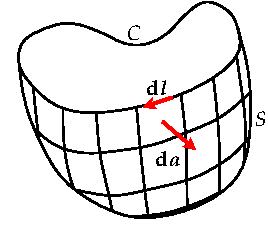
\includegraphics{Imatges/Stokes.pdf}
\caption{Conveni de signes del teorema d'Stokes}
\label{pic:signe-teo-stockes}
\end{figure}

\end{document}
